%% 
%% Copyright 2007, 2008, 2009 Elsevier Ltd
%% 
%% This file is part of the 'Elsarticle Bundle'.
%% ---------------------------------------------
%% 
%% It may be distributed under the conditions of the LaTeX Project Public
%% License, either version 1.2 of this license or (at your option) any
%% later version.  The latest version of this license is in
%%    http://www.latex-project.org/lppl.txt
%% and version 1.2 or later is part of all distributions of LaTeX
%% version 1999/12/01 or later.
%% 
%% The list of all files belonging to the 'Elsarticle Bundle' is
%% given in the file `manifest.txt'.
%% 

%% Template article for Elsevier's document class `elsarticle'
%% with numbered style bibliographic references
%% SP 2008/03/01

\documentclass[preprint,12pt]{elsarticle}
\usepackage{mathtools}

%% Use the option review to obtain double line spacing
%% \documentclass[authoryear,preprint,review,12pt]{elsarticle}

%% Use the options 1p,twocolumn; 3p; 3p,twocolumn; 5p; or 5p,twocolumn
%% for a journal layout:
%% \documentclass[final,1p,times]{elsarticle}
%% \documentclass[final,1p,times,twocolumn]{elsarticle}
%% \documentclass[final,3p,times]{elsarticle}
%% \documentclass[final,3p,times,twocolumn]{elsarticle}
%% \documentclass[final,5p,times]{elsarticle}
%% \documentclass[final,5p,times,twocolumn]{elsarticle}

%% For including figures, graphicx.sty has been loaded in
%% elsarticle.cls. If you prefer to use the old commands
%% please give \usepackage{epsfig}

%% The amssymb package provides various useful mathematical symbols
\usepackage{float}
\usepackage{amssymb,natbib}
%% The amsthm package provides extended theorem environments
%% \usepackage{amsthm}

%% The lineno packages adds line numbers. Start line numbering with
%% \begin{linenumbers}, end it with \end{linenumbers}. Or switch it on
%% for the whole article with \linenumbers.
%% \usepackage{lineno}

\journal{Knowledge Based Systems}

\begin{document}

\begin{frontmatter}

%% Title, authors and addresses

%% use the tnoteref command within \title for footnotes;
%% use the tnotetext command for theassociated footnote;
%% use the fnref command within \author or \address for footnotes;
%% use the fntext command for theassociated footnote;
%% use the corref command within \author for corresponding author footnotes;
%% use the cortext command for theassociated footnote;
%% use the ead command for the email address,
%% and the form \ead[url] for the home page:
%% \title{Title\tnoteref{label1}}
%% \tnotetext[label1]{}
%% \author{Name\corref{cor1}\fnref{label2}}
%% \ead{email address}
%% \ead[url]{home page}
%% \fntext[label2]{}
%% \cortext[cor1]{}
%% \address{Address\fnref{label3}}
%% \fntext[label3]{}

\title{ML-MS Studio: A Generic Free and Open-Source Tool for Mass Spectrometry Analysis and Classification}

%% use optional labels to link authors explicitly to addresses:
%% \author[label1,label2]{}
%% \address[label1]{}
%% \address[label2]{}

\address[addr1]{Bioinformatics - UFPR}
\address[addr2]{Biochemistry - UFPR}

\author[addr1]{Calebe Elias Ribeiro Brim }
\author[addr1]{Roberto Tadeu Raittz}
\author[addr2]{Luciano Uergo}


\address{}

\begin{abstract}
%% Text of abstract
Mass spectrometer is a useful tool for biochemistry research field analysis. It is used to identify microorganisms, protein, chemical compounds and complex diseases by blood analysis. There is many tools and libraries to handle different steps of mass spectrometry (MS) data analysis. However, the integration of all these tools lacks user friendly approaches. We developed a machine learning solution capable to handle all steps of MS data analysis. The ML-MS Tool is an free software that integrate different mass spectrometry analysis techniques with machine learning approach. We focused in automatic feature extraction, avoiding the need of manual peaks analysis of biomarkers. With all feature extracted ML-MS versatile classification tool avoiding the need reprocess the new MS samples. ML-MS is divided into two sub-products, the ML-MS Tool and the ML-MS Library; both products are free and open source. The ML-MS Library is focused on script routines, that might be used integrated to another automated scripts. And ML-MS Tool is focused on final users avoiding the knowledge about programming language. With ML-MS library we can reach values greater of than 97-100\% of accuracy for Ovarian Cancer QA/QC serum proteomics data-set.


\end{abstract}

\begin{keyword}
%% keywords here, in the form: keyword \sep keyword

%% PACS codes here, in the form: \PACS code \sep code

%% MSC codes here, in the form: \MSC code \sep code
%% or \MSC[2008] code \sep code (2000 is the default)
Machine Learning,
Feature Extraction,
Mass Spectrometry,
Peak Picking



\end{keyword}

\end{frontmatter}

%% \linenumbers

%% main text
\section{Introduction}
\label{sec:introduction}

The Mass Spectrometry (MS) analysis has widespread concept on proteomic research field. Since the beginning of mass spectrometry analysis the scientists seek for an effective way to use MS analysis, as a precise diagnostic tool. High-resolution mass spectrometry technique has better results for diagnosis because of amount of information generated \cite{Levner2006}. 

The great amount of data is also needed an better feature extraction strategy to reach good learning rates; according Tirumalai an accurate distinction of differences between mass spectrometry data are only possible considering m/z and its respectively intensities  \cite{Tirumalai2003}.

This article will approach the peak picking \cite{Swan2013}, this strategy avoid the need of peaks biological identification and is focused on signal processing.    


Mass spectrometry data is handled by methods of different fields, some based on statistical, mathematics or artificial intelligence approach. With the increase of number of available methods the complexity of use this tools is also increased turning it out unreachable. Seeking for a tool that works with high number of features we could not find anything useful; Shen et. All\cite{Shen2007} also report an problem to find a tool that complains these requirements; so we propose Machine Learning Mass Spectrometry (ML-MS), a generic free and open-source tool to process high dimensional mass spectrometry data, focused classification task. ML-MS can handle all analysis and diagnostic process:

\begin{itemize}
\item pre-processing;
\item peaks selection;
\item biomarker finder;
\item feature extraction and
\item classification.
\end{itemize}


All feature extraction  strategies and biomarker selection are focused on generate high correlated 'features' to improve the classification task.
 
Inspired on Petricoin\cite{Petricoin2002} we use evolutionary algorithms we develop two main feature extractor algorithm: Watch Points and Feature Resonance

 We develop a free and open source software focused on machine learning approach; ML-MS is based on supervised learning and feature extraction, where a set of labeled samples are used on feature extraction and training process . On automatic feature extraction process we use genetic algorithm (GA), that is an evolutionary algorithm used to perform a best solution for an problem; to evaluate those solutions we use correlation measure to define which one is the best feature extraction configuration. 
 

\begin{figure}[H]
\centering
    %\reflectbox{%
    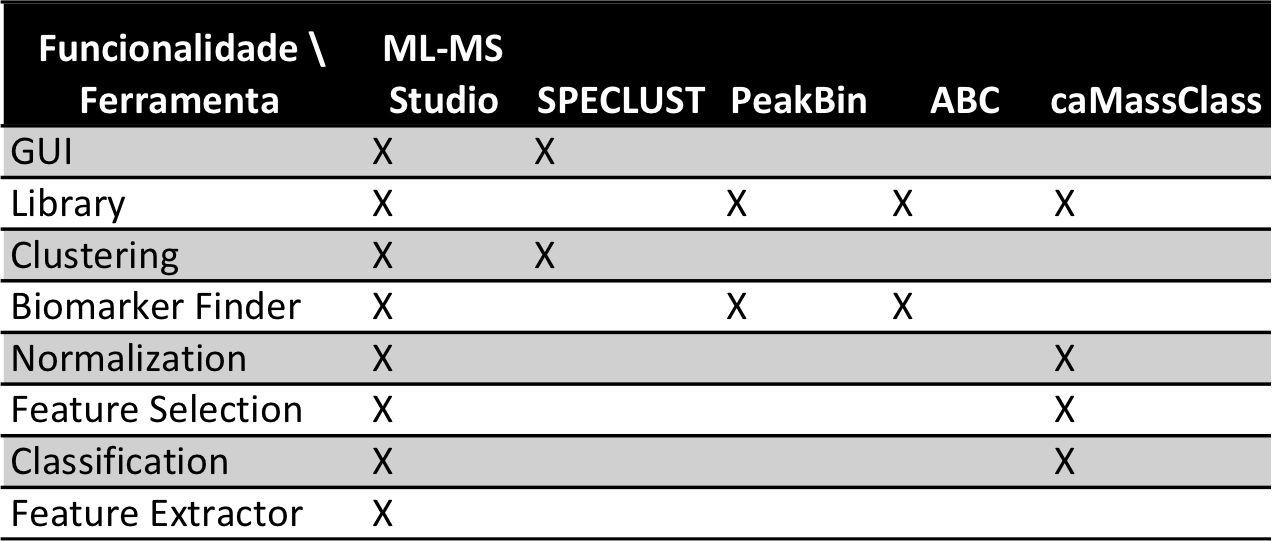
\includegraphics[width=0.7\textwidth]{images/funcionality_comparison.png}
    %}
    \caption{MS-ML Studio comparison exceeded in functionality all compared tools}
    \label{fig:functioncompariosn}
\end{figure}
The figure \ref{fig:functioncompariosn} show some tools used to process mass spectrometry data and how ML-MS fill up the some gaps of functionality presented on conventional MS data processing tools\cite{Henson2004}\cite{Johansson2006}\cite{Armananzas2011}\cite{Shen2007}.

 \subsection{Correlation Analysis}



To understand how is the behavior of correlation feature extraction, first  is needed to understand how the correlation work. The use of correlation is widespread concept on biological and feature extraction analysis field\cite{Katchalski-katzirtt1992}\cite{Cox2008}. Because of Increase of the data dimensionality the feature selection is an very important step to remove redundant and irrelevant features that could reduce the learning performance of machine learning algorithms\cite{Yu2003}. According Lei Yu and Huan Liu \cite{Yu2004} the correlation measure is widely used in machine learning  and statistics to show the strength of feature (Sections: \ref{subsec:watchpoints} and \ref{subsec:featureresonanse}).


 

The correlation measure is the backbone of this work used to measure the relevance of all features. During the feature extraction process correlation is used by the GA to generate high correlated features.  

\section{Materials and Methods}

We develop a generic tool capable to handle different types of Mass Spectrometer, using as basement the Ovarian Cancer Post QAQC data set (provided by Clinical Proteomic Program - http://home.ccr.cancer.gov/ncifdaproteomics/ppatterns.asp). All data are generated from blood samples of healthy and diagnosed Ovarian Cancer women.

We embed an optional align algorithm on the case to import unaligned samples; Iconshift is a free and open-source alignment algorithm originally developed to align chromatographic data. The tests realized with mass spectrometry data it is also capable to process equally\cite{Tomasi2011}.

\begin{figure}[H]

    \centering
    %\reflectbox{%
    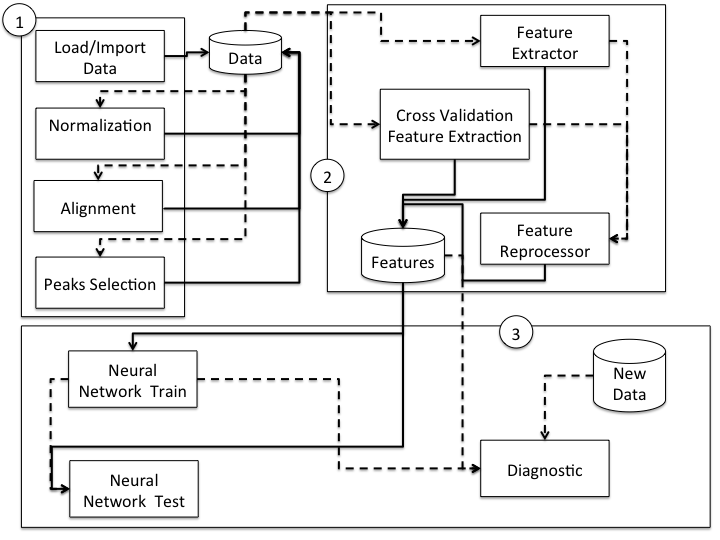
\includegraphics[width=0.7\textwidth]{images/workflow_chart.png}
    %}
    \caption{ML-MS workflow is divided in three main general section. The section 1 represent data pre-processing where all data is normalized all peaks aligned and selected. The section 2  represent all types of feature extraction that can be used. The section 3  is about  machine learning and the consolidation of diagnostic tool, where new unclassified data will be classified (Author 2015).}
    \label{fig:workflow}
\end{figure}
The figure \ref{fig:workflow} represents all steps of ML-MS workflow. The next sections will explain each of those steps detailed and finishing on figure \ref{fig:workflow}.3

\subsection{Load and Import Data}


The data preprocessing consists in prepare the raw data to shape the system definitions. Figure \ref{fig:workflow}.1 is formed by four main steps. The import/load of data is the beginning of preprocessing data, this step bring the raw data into our system format and start to work with this data. Note that this step is only available on MS-ML Software. The user that work with MS-ML Library should manage spectrum data by themselves.

\subsection{Normalization}
As much higher resolution of spectrum is as so is the machine processing time and the complexity of analysis. To solve this problem and satisfy all workflow problems we create 2 buttons on MS-ML Software: the Normalization and the Re-shaping button; both process are based on normalization process. The normalization button is relative to intensity values of spectrum and for each spectrum the is:

\begin{equation}
N(x) = x_i - \min(x)/max(x)-\min(x)
\end{equation}


\subsection{Peaks Selection}
\label{subsec:peaksselection}

The peaks selection strategy is the first step for MS analysis; on this step the real peaks are differed from the spectral noise. The fuzzy moving average (FMA) strategy can be set to be specific, selecting the smaller peaks, or general, selecting only more expressive peaks; different configurations on peaks selection can impact on correlation on automatic feature extraction process. Considering that 'x' is all possible intensity values on spectrum the peaks selection process is leaded by following equations: 

\begin{equation}
S(x;p,w) = \frac{\sum_{i=p-w}^{p+w}(x_{i}  T(2w+1,i))}{2w+1}
\end{equation}
having:

\begin{equation}
	p\ \epsilon\ N^*|\  1\leq p-w,\ p+w \leq S
\end{equation}


Where 'p' is the m/z vector index; 'w' is the half window size minus one; and 'x' is the vector of intensities; 'i' represents the window index and 'T' is an triangular function that receive the size and the respective window indexer 'i'. 

The peaks selection process generate three main vectors: 

\begin{enumerate}
\item idx - The 'idx' is a logical vector with same size of spectrum where is marked with one (1)  if the peaks selection algorithm find a peak and zero otherwise;
\item selected\_mz - selected m/z value;
\item selected\_ii - selected intensities. 
\end{enumerate}



\subsection{Feature Extraction}
\label{subsec:featureextraction}
The feature extraction is based on data transformation. A good feature extraction imply in a good correlation with respective classes and high scores on learning algorithms. To avoid over-fitting on feature extraction process, on GA based feature extraction uses validation procedure as is showed on figure:\ref{fig:validation}.


\begin{figure}[H]
    \centering
    %\reflectbox{%
    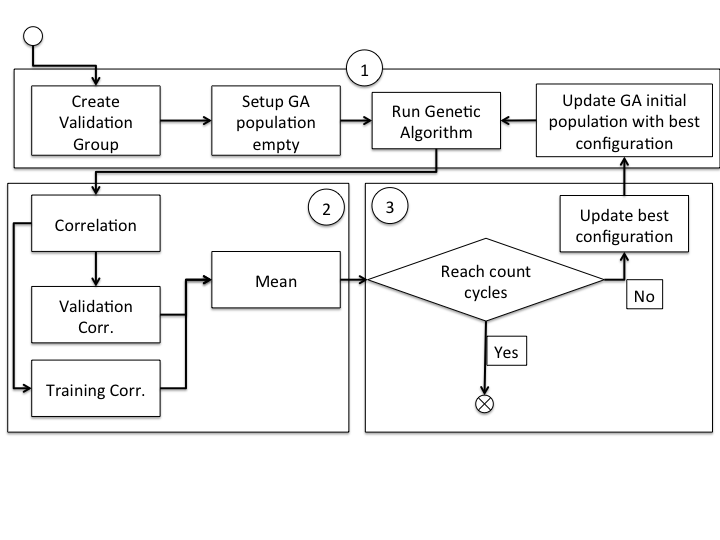
\includegraphics[width=0.7\textwidth]{images/cross_validation_workflow.png}
    %}
  	\caption{Work-flow of all  validation based functions. The section 1 represents the setup of GA settings as well creation of two groups from training set moving some samples to validation group; this section is where the feature extraction happen. After the execution of GA, the feature extractor, the section 2 represent the validation of feature extracted; The correlation step measure the correlation of selected features with its respectively classes for both groups, training and validation data sets. If the mean of training and validation correlations increase from past run the algorithm will assume that the current feature configuration is the best general feature. The section 3 represent the stop condition, that can be the cycles count or count of the same features generated consecutively (Author 2015).}
\label{fig:validation}
\end{figure}


\subsection{Best Peaks Selection}
\label{subsec:bestpeaksselection}
The Best Peaks Selection is the procedure that choose between the selected peaks the best ones. There is two methods to make this selection:

\begin{itemize}
\item Correlation: Measure the correlation of 'idx' vector (Section: \ref{subsec:peaksselection}), on the peaks selection method, with its respectively classes.
\item Probability Based: Measure the difference of peak existence probability for all classes.
\end{itemize}

 For both methods the user must choose an cut-line value; only peaks with values greater than cut-line is selected as best peak on algorithm selection process.


\subsection{Watch Points}
\label{subsec:watchpoints}

The watch points technique is focused to generate features to express the importance of neighborhood peaks. The watch points use fuzzy logic, where each watch point is a triangular weight window \ref{fig:weightedwindows}


\begin{figure}[H]
    \centering
    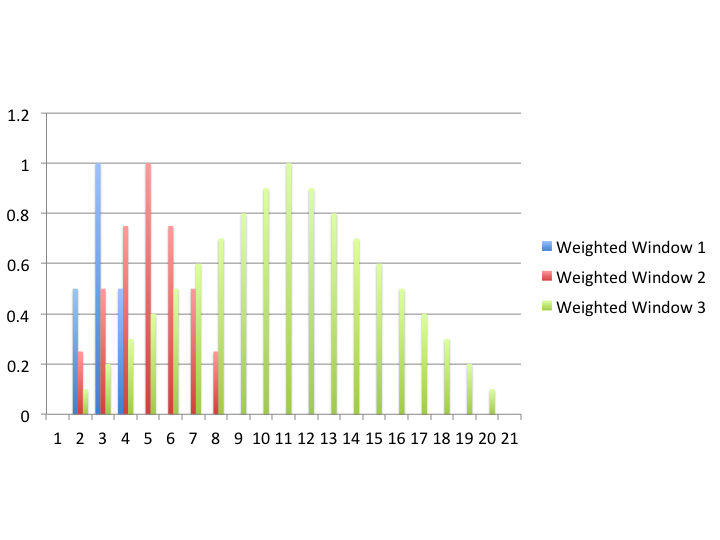
\includegraphics[width=0.7\textwidth]{images/weightedwindow.png}
  	\caption{Representation of envelope of watch-points; those three watch-points have different centers and distances. Different distances imply on differences on wheight granularity (Author 2015).}
    \label{fig:weightedwindows}
\end{figure}

On figure \ref{fig:weightedwindows} considering three different watch points ( blue, red and green). An watch point have different size and weight distribution.  The triangular function is expressed by following equation \ref{eq:triangfunc}.


For L odd:
\begin{equation}
\label{eq:triangfunc}
w (n) =\left\{\begin{matrix}
2n/L+1  & 1 \leq n \leq (L+1)/2 \\  
 2-2n/L+1  & (L+1)/2+1\leq n \leq L 
\end{matrix}\right.
\\
\\
\end{equation}
For L even:

\begin{equation}
w(n) = \left\{
\begin{matrix}
	(2n-1)/L & 1 \leq n \leq L/2\\ 
	2-(2n-1)/L & L/2+1\leq n \leq L
\end{matrix}\right.
\end{equation}

The watch point feature extraction process is based on validation procedure showed on figure \ref{fig:validation}. The fitness function that leads the evolutionary algorithm is expressed on figure: \ref{fig:watchfitness}

\begin{figure}[H]
    \centering
    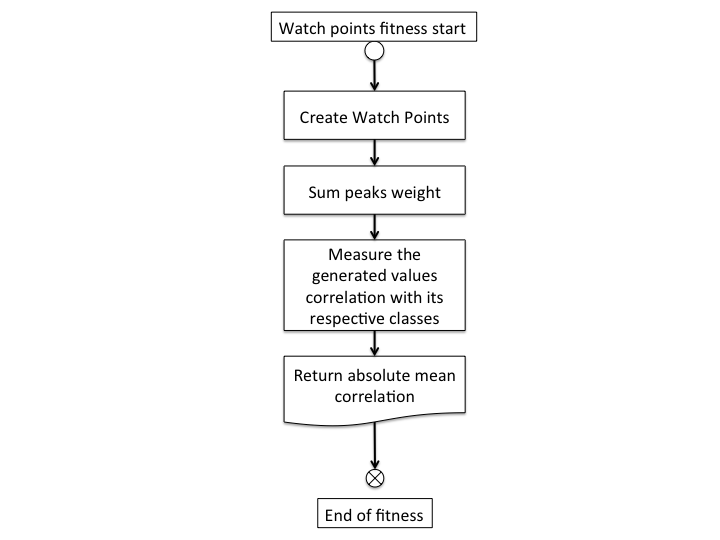
\includegraphics[width=0.7\textwidth]{images/watchpoint_fitness.png}
  	\caption{The Watch point fitness workflow generate a sum of all peaks weights relative to each watch-point.(Author 2015).}
    \label{fig:watchfitness}
\end{figure}

The best peaks selection process is used to choose the bests watch points centers but is the evolutionary algorithm GA is responsible to determine the watch points distances. The feature extractor automatically optimize the best distances for each selected centers. The second step on the fitness function is based on sum of all weights. Considering that 'w' is the watch point universe expressed by the triangular function \ref{eq:triangfunc} on page \pageref{eq:triangfunc} and 'p' is the 'idx' vector of peaks selection  \ref{subsec:peaksselection} the sum of peaks weights is leaded by following equation:

\begin{equation}
y  = \sum w*p
\label{eq:watchpoints}
\end{equation}

Where 'y' is generated for each watch point and for all spectrum samples, where 'w' and 'p' has the same size. The next step is the measure of all features correlation with its respectively classes and the result is the mean module correlation of all watch points. 

\subsection{Feature Resonance}
\label{subsec:featureresonanse}

\begin{figure}[H]
    \centering
    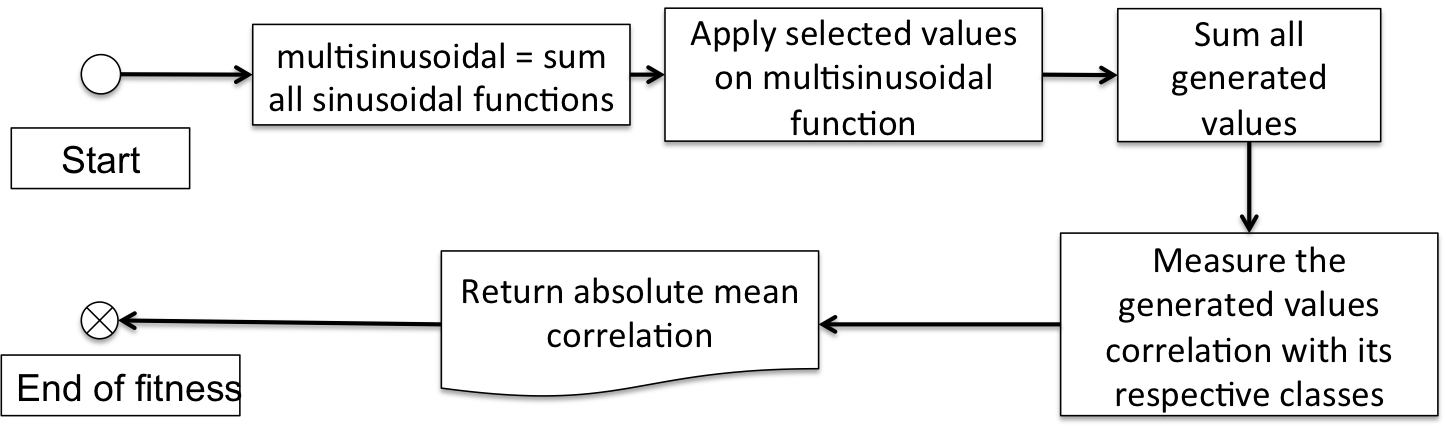
\includegraphics[width=0.7\textwidth]{images/feature_resonanse_workflow.png}
  	\caption{Representation of feature resonance fitness function. The ‘multisinusoidal’ variable receive the sum of all sinusoidal functions; the graphic representation of ‘multisinusoidal’ function is represented on figure \ref{fig:sinusoidalpos} its general on equation \ref{eq:sumsinusoids} (Author 2015).}
    \label{fig:resonansefitness}
\end{figure}

The Feature Resonance is also validation based feature extractor. The main purpose of this feature extraction is generate values based on one or more sinusoidal functions. The figure \ref{fig:sinusoidalpos} represent sinusoidal function with one, two and three waves respectively and the red circles represents the values passed to the feature extractor.  

\begin{figure}[H]
    \centering
    %\reflectbox{%
    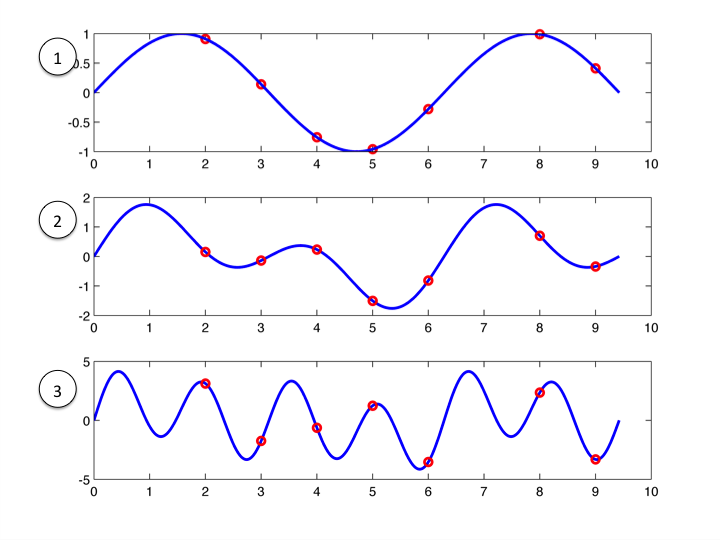
\includegraphics[width=0.7\textwidth]{images/sin_and_pos.png}
    %}
  	\caption{This is an simplified example of how feature resonance extractor works. The function 1 is a simple sinusoidal function where the red circles represent the function domain. The function 2 represent the sum of two sinusoidal functions and the function 3 represent an sum of three sinusoidal functions. Different configurations of frequency and amplitude can generate different values to the same peaks set (Author 2015).
}
\label{fig:sinusoidalpos}

\end{figure}
The Feature Resonance can extract information of m/z values or its respectively intensity by the same way expressed on the following equation:
\begin{equation}
\label{eq:sumsinusoids}
w  = \sum_{i = 1}^M\sum(a_i*\sin(b_i+c_i*x ))
\end{equation}

Where 'w' is the feature value; 'a', 'b' and 'c' are provided by the GA; 'x' is the provided values, 'M' is the number of waves set by user and \(i\ E\ N^*\).  Then the correlation value is measured and returned the module of correlation to genetic algorithm.

There is some variants of feature resonance feature extractor where the same algorithm could process the intensities and m/z values. There is a another variant that process only information over the specified the watch-points. 

\section{Results}
\label{sec:results}
\subsection{ML-MS Studio \& ML-MS Library}

\subsubsection{The Library}
Our main results of this research is the ML-MS Studio and Library; this is a complete machine learning tool for mass spectrometry processing and classification. The ML-MS Studio is based on ML-MS Library which all functions used on ML-MS Studio is on MS-ML Library. The advantage to use ML-MS Studio against MS-ML Library is the practically to import and handle the data without programming Knowledge. The MS-ML Studio is focused to attend the conventional routines and the ML-MS Library is focused on bioinformatician researchers to integrate with other tools and give an greater control over non conventional routines that can be viewed on figure \ref{fig:msmllibrarystruct}. 

\begin{figure}[H]
    \centering
    %\reflectbox{%
    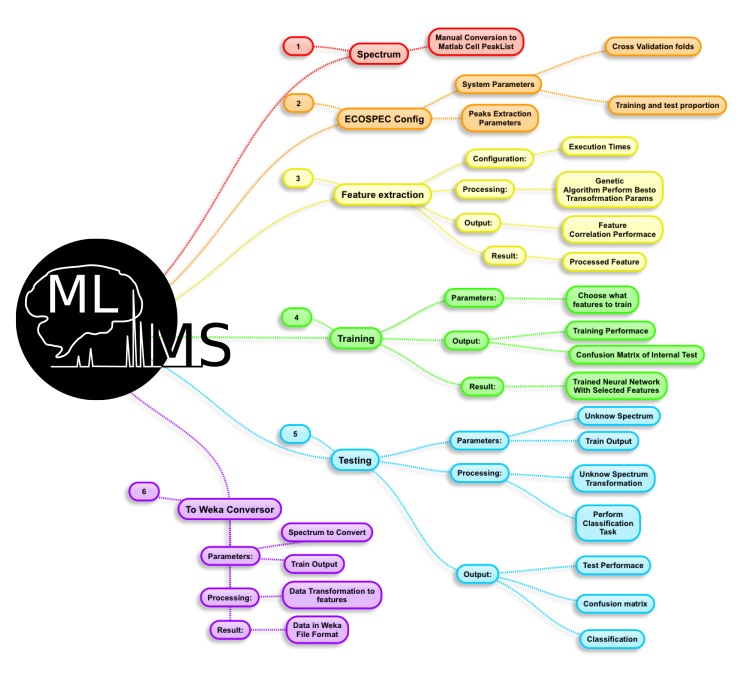
\includegraphics[width=0.7\textwidth]{images/LibraryStructure.png}
    %}
  	\caption{This figure show the principals functionality of MS-ML Library (Author 2015).}
\label{fig:msmllibrarystruct}

\end{figure}

The ML-MS Library handle the preprocessing and post processing procedures and all steps of machine learning procedure, that includes feature extraction, training and testing routines. 







\subsubsection{The Studio}
\begin{figure}[H]
    \centering
    %\reflectbox{%
    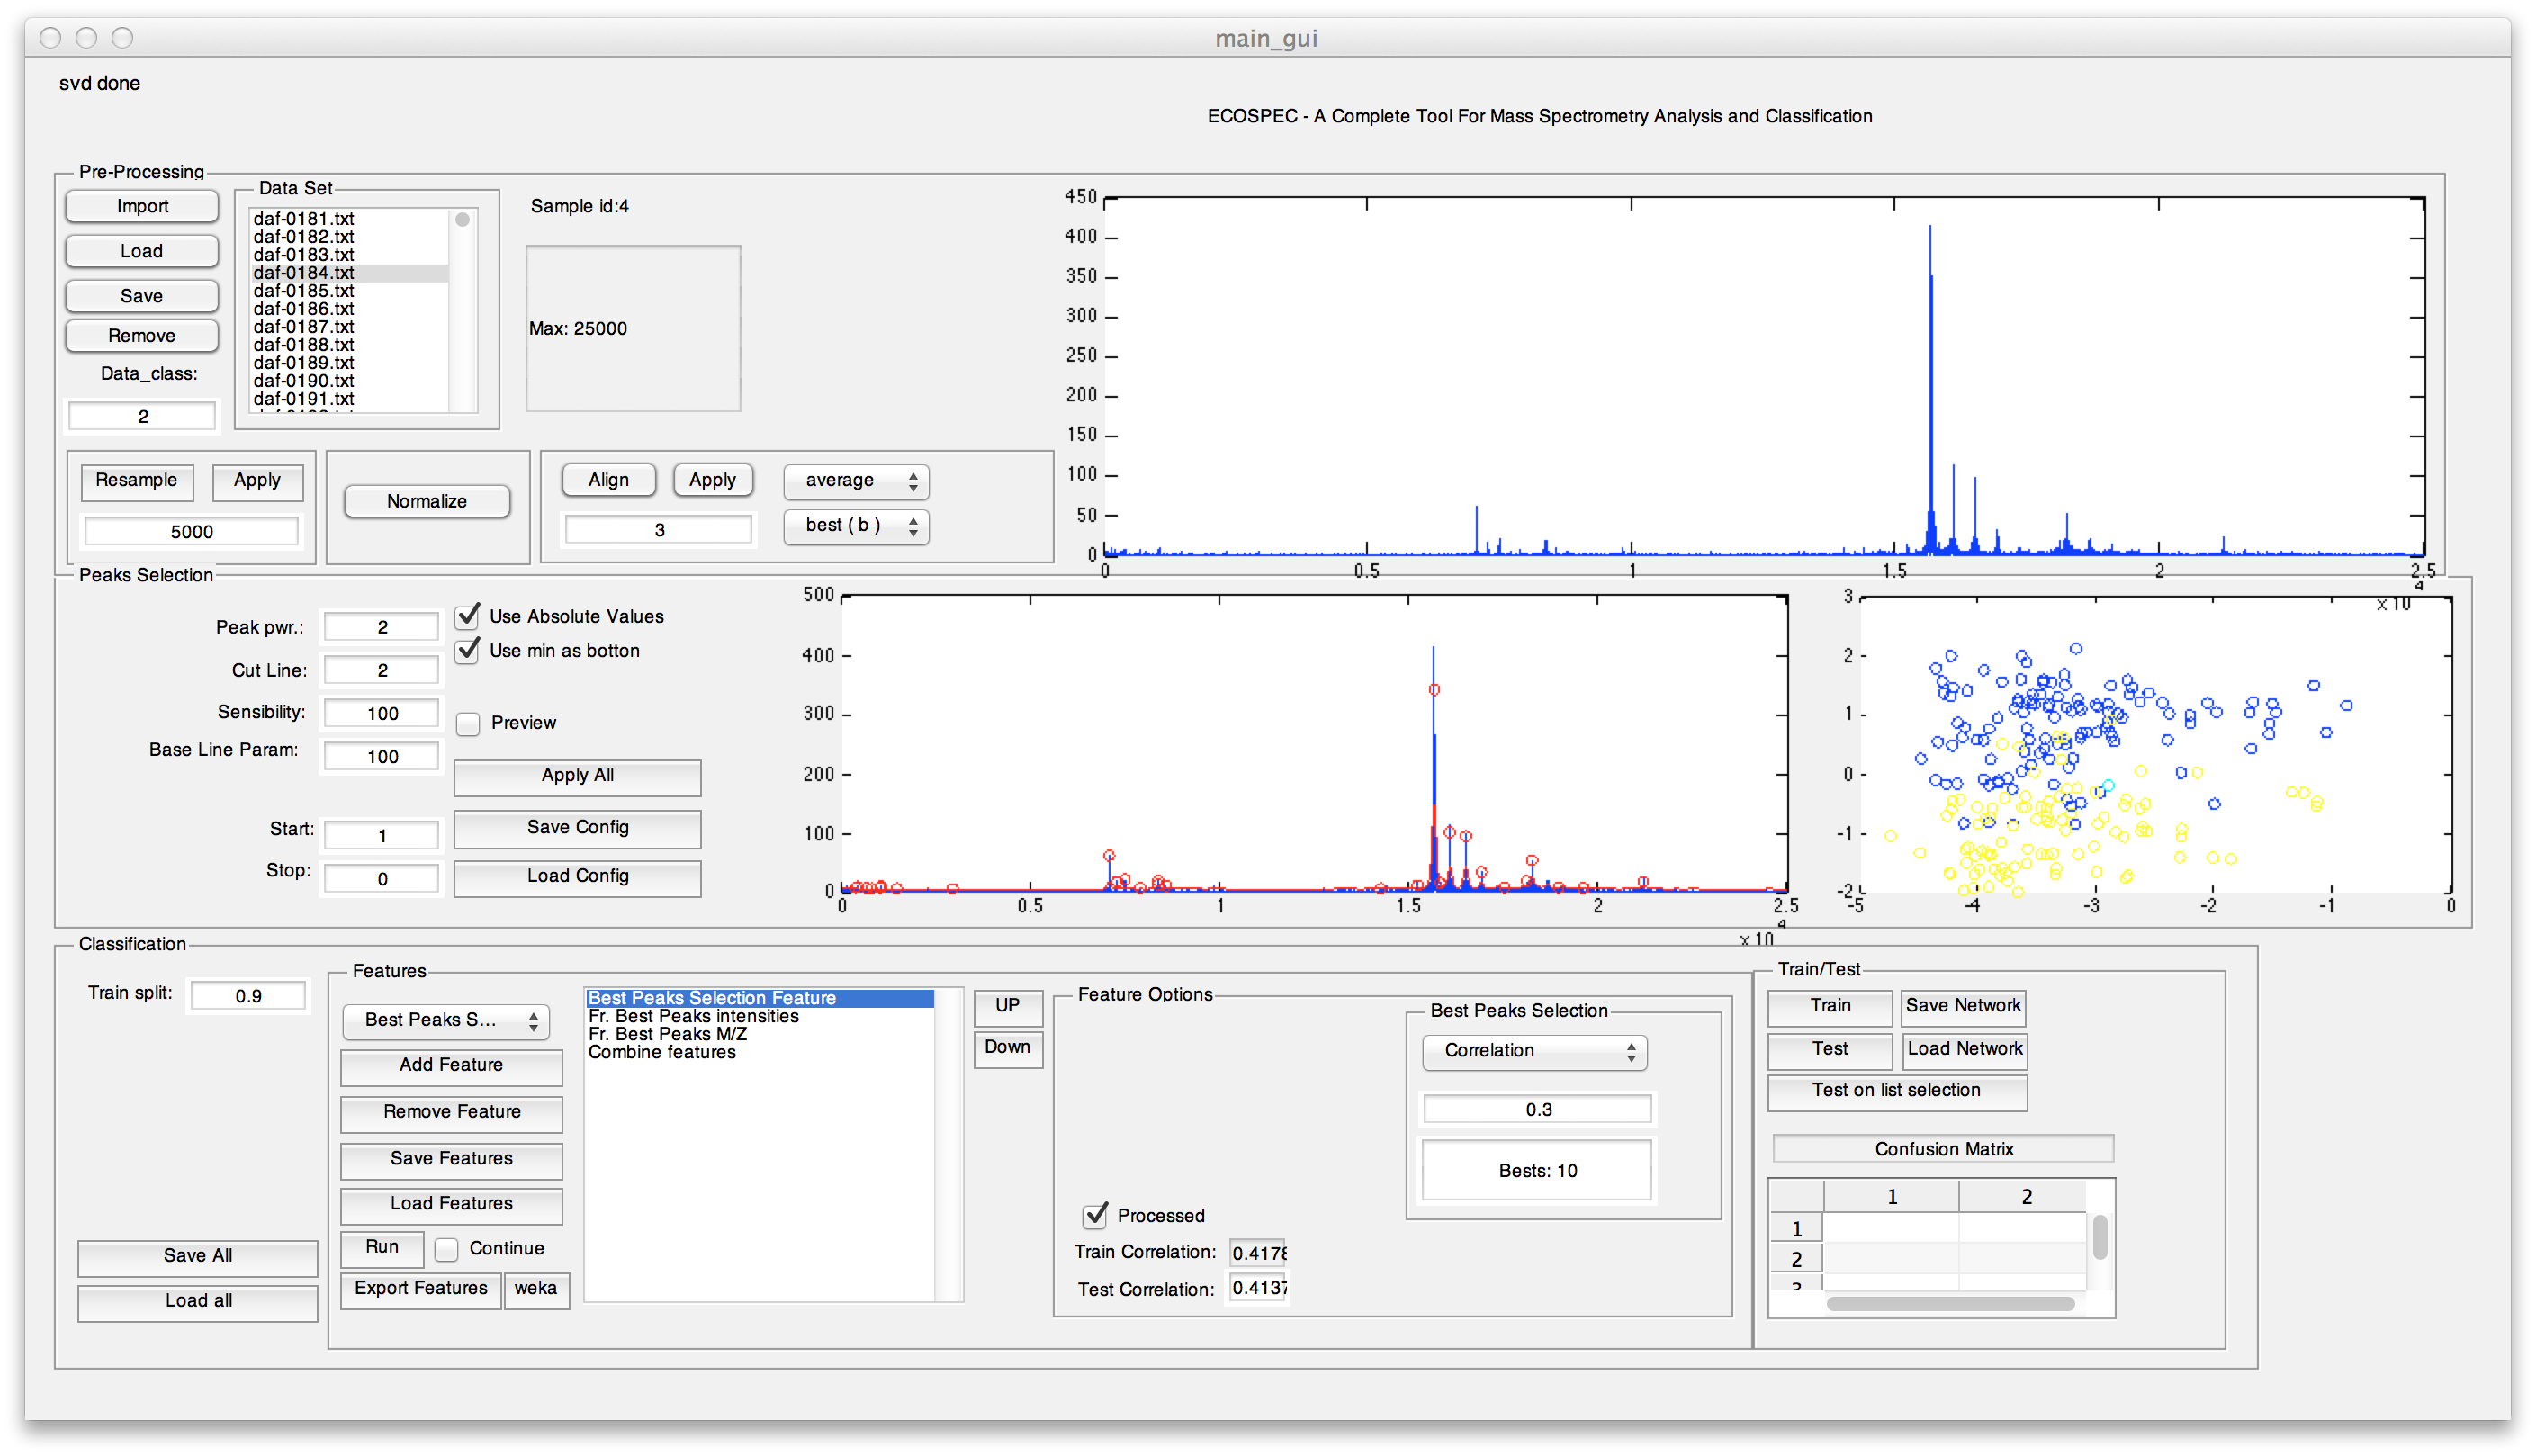
\includegraphics[width=0.7\textwidth]{images/Full_GUI.png}
    %}
  	\caption{This figure shows the GUI of ML-MS Studio working with Ovarian Cancer data-set (Author 2015).}
\label{fig:fullgui}

\end{figure}
The ML-MS Studio Was developed focused on simple usability and ergonomic design. As can be seen on figure \ref{fig:fullgui} exists three main division on GUI; The first panel is excursively to data pre-processing where user can import, save, load and change the number classification of each data.

\subsection{Ovarian Cancer Serum Proteomics QA/QC }
To measure the feature efficiency we use as comparison parameter an Ovarian cancer study. For the data-set "Ovarian Cancer serum proteomics QA/QC" previously used by Conrads\cite{Conrads2004}, was possible to reach the values of 100\% of Sensitivity and Specificity (Figure: \ref{tbl:comparisonresults}).

\begin{figure}[H]
    \centering
    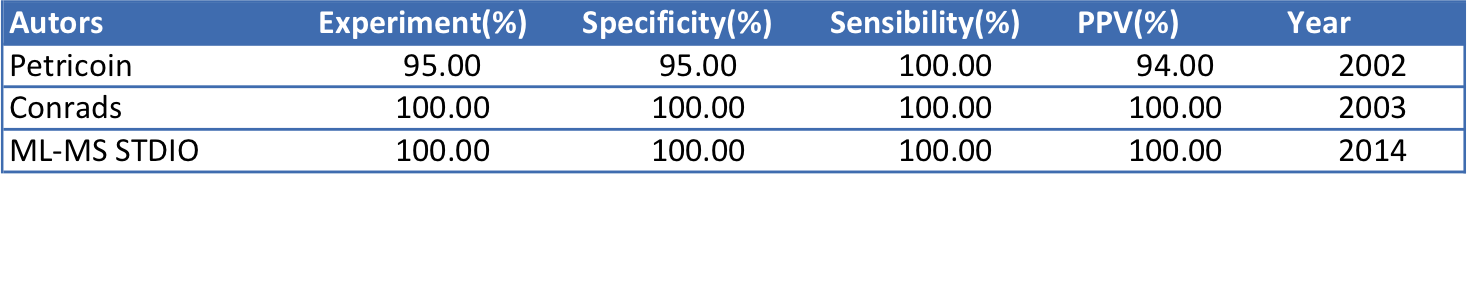
\includegraphics[width=0.7\textwidth]{images/Comparison_Table.png}
    \caption{Comparison of original Positive Predictive Value (PPV) Precision (Sensibility) and Accuracy (Specificity)  and the results acquired with MS-ML Studio (Author 2015).}
\label{tbl:comparisonresults}
\end{figure}


The figure\ref{tbl:comparisonresults}  using different techniques on the same data-set ML-MS STDIO was capable to reach the same original scores\cite{Petricoin2002}\cite{Conrads2003}. To reach this results was used a set of feature extractors developed on ML-MS STDIO, testing each feature with empirical method. The resolution of QA/QC data-set was reduced from 360k m/z values to of 15k m/z values, reducing the use of computational resources like memory and storage. The watch points feature extractor was used with best peaks selection with correlation cut-line 0.3, running by hundred cycles. The best peaks selection feature extractor was used with peaks crossing the cut-line of  0.2 and 0.3 of correlation. The feature resonance feature extractor was used with best peaks selection with correlation cut-line of 0.3 correlation to process m/z values and intensity values with hundred times and twenty waves. The feature resonance also reprocess the m/z values over the watch point feature extractor area with correlation of 0.3 cut-line. All feature extracted was processed on MLP machine learning algorithm.


\subsection{Prostate Cancer Results}

We also run some tests on prostate cancer data-set. The Prostate Cancer data-set (provided by Clinical Proteomic Program -  home.ccr.cancer.gov/ ncifdaproteomics/ ppatterns.asp) is divided into four main groups:

\begin{enumerate}
\item Normal;
\item Benign PSA Greater than 4;
\item PSA 1-4 and
\item PSA Greater than 4.
\end{enumerate}

We apply same methodology used on Lilien\cite{Lilien2003} experiments classifying  all data into 2 and 3 groups, BC ( Benign and Cancer ) and NBC (Normal, Benign and Cancer). On BC Group we reach 0.90 of accuracy and 100\% of precision using MS-ML Studio with three features extractors; each feature extractor reach an men 0,6 of Pearson Correlation; those three features are processed using the m/z values with correlation greater than 0,12.  


\subsection{Intact Cell Microorganism}



The intact cell experiments was made with Microorganisms of Aeromonas family. All these experiments are made on Brucker MALDI-TOF analyzer. The data and bacterial sample preparation procedure and the original experiment can be found at Surek 2010 \cite{Surek2010}. For identification experiment we use one against all strategy, were each class of microorganism is tested against the others. The samples used on these test contain four bacteria: 

\begin{itemize}
\item A. veronii/sobria;
\item A. cavie;
\item A. hidrophilla
\item A. trota
\end{itemize}


And the following groups was generated: 

\begin{enumerate}
\item  A. veronii/sobria against all;
\item  A. cavie against all;
\item  A hidrophilla against all;
\item and A. trota against all
\end{enumerate}

These four groups generate four experiments; for each experiment  90 percent of samples are used for the feature extraction task and the target class was set as number one and the other classes as number two. The results for each group is represented on figure \ref{tbl:resultaero}


\begin{figure}[H]
    \centering
    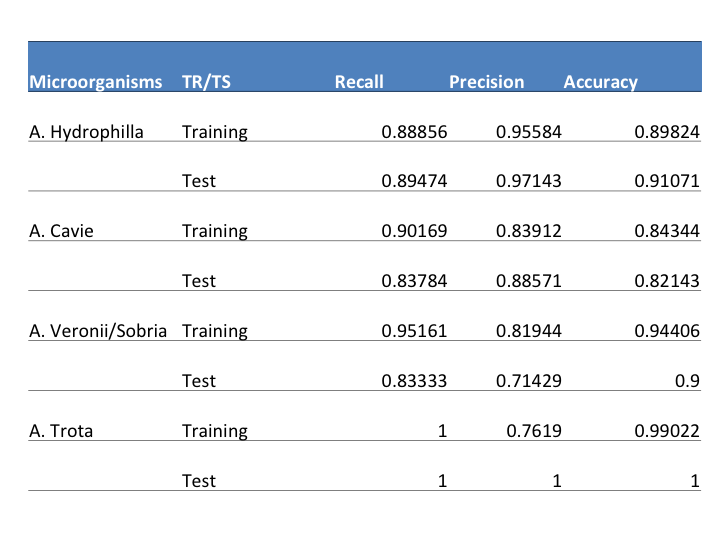
\includegraphics[width=0.7\textwidth]{images/AeromonasScore.png}
    \caption{Precision measures achieved with ML-MS Studio for each  four Aeromonas groups (Author 2015).}
\label{tbl:resultaero}
\end{figure}



\subsubsection{A. Veroni/Sobria Results}
The group "A.Veronii/Sobria against all" we use: "FR Selected M/Z" resulting in features with 0.67 of correlation with classes, "FR Best Peaks Intensity" with correlation threshold of 0.18 generating feature values with 0.66 of correlation and "FR Best Peaks m/z" with correlation threshold of 0.12, 0.16, 0.2 and 0.25 generating features with correlation 0.77, 078, 0.48, 0.63. 
We create figures \ref{fig:pcaveronisobriacomparison} \ref{fig:pcacaviecomparison} \ref{fig:pcahidrophilacomparison}  with purpose to show graphically the performance of ML-MS Studio feature extractors. Is possible to see clearly that after feature extraction is information is much more representative. 

  \begin{figure}[H]
    \centering
    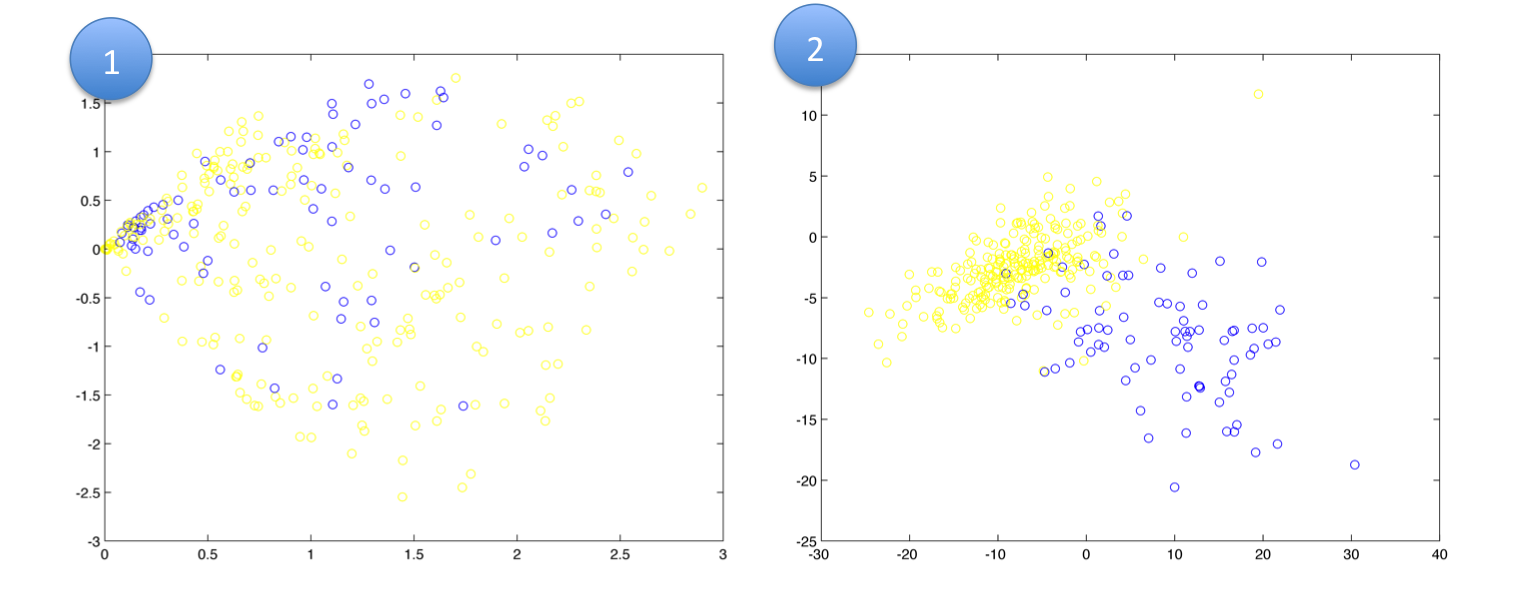
\includegraphics[width=0.7\textwidth]{images/Comparison_PCA_VeroniSobria.png}
    \caption{Both images are an made with ML-MS Studio applying PCA analysis with two classes. Figure number one represents PCA technique with only m/z values of selected peaks; figure two represents the PCA analysis made with feature extraction. The blue circles represents A.Veronii/Sobria samples and the yellow ones are the other samples. (Author 2015).}
\label{fig:pcaveronisobriacomparison}
\end{figure}

\subsubsection{A. Cavie Results}
For "A.Cavie against all" group we use "FR. selected M/Z" feature extractor; "Fr. Best Peaks M/Z" with correlation threshold of 0.12, 0.16, 0.2 and "Fr. Best Peaks Intensities" with correlation threshold of 0.18. The PCA representation for "A.Cavie against all" is represented on figure \ref{fig:pcacaviecomparison}.

  \begin{figure}[H]
    \centering
    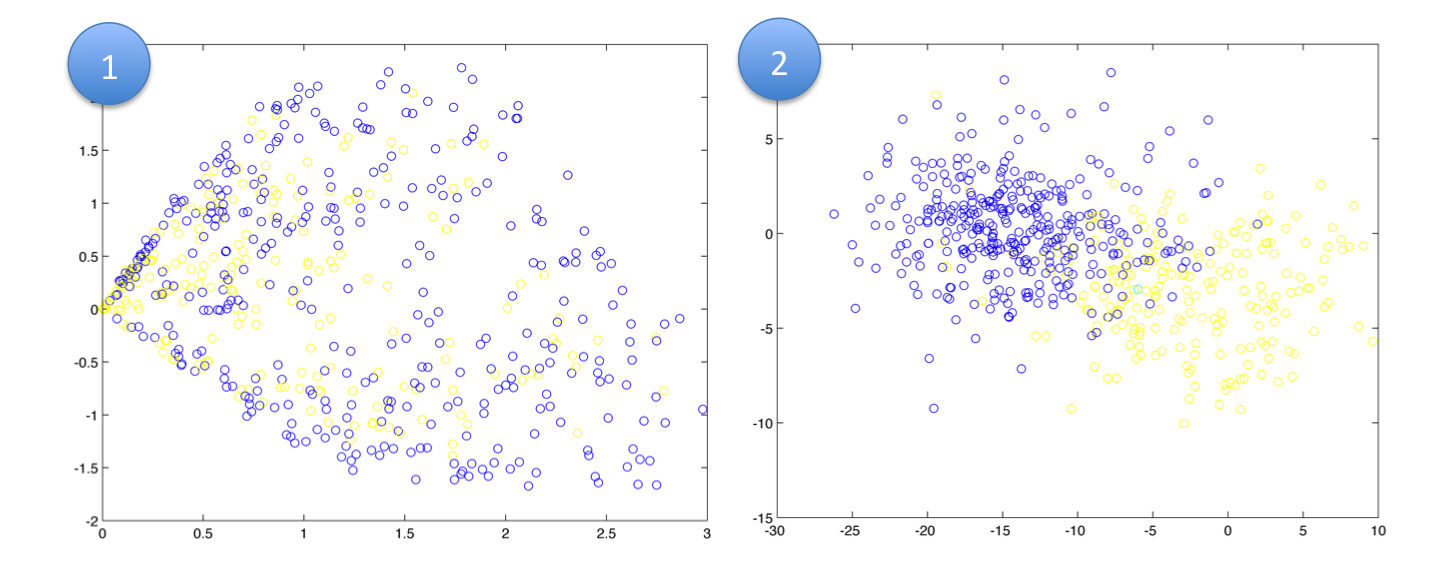
\includegraphics[width=0.7\textwidth]{images/Comparison_CAVIE_PCA.png}
    \caption{Both images are an made with ML-MS Studio applying PCA analysis with two classes. Figure number one represents PCA technique with only m/z values of selected peaks; figure two represents the PCA analysis made with feature extraction. The blue circles represents A.Cavie samples and the yellow ones are the other samples. (Author 2015).}
\label{fig:pcacaviecomparison}
\end{figure}
\subsubsection{A. Hydrophilla Results}
For the "Hydrophilla against all" group,  we use FR. Best Peaks MZ Feature extraction with best peaks selection correlation threshold 0.11, 0.12, 0.15 and 0.16 generating features with correlation 0.66, 0.64, 0.57 and 0.56 for the training set. The figure\ref{fig:pcahidrophilacomparison} represents the PCA distribution of feature extracted and the selected peaks. 
  
  \begin{figure}[H]
    \centering
    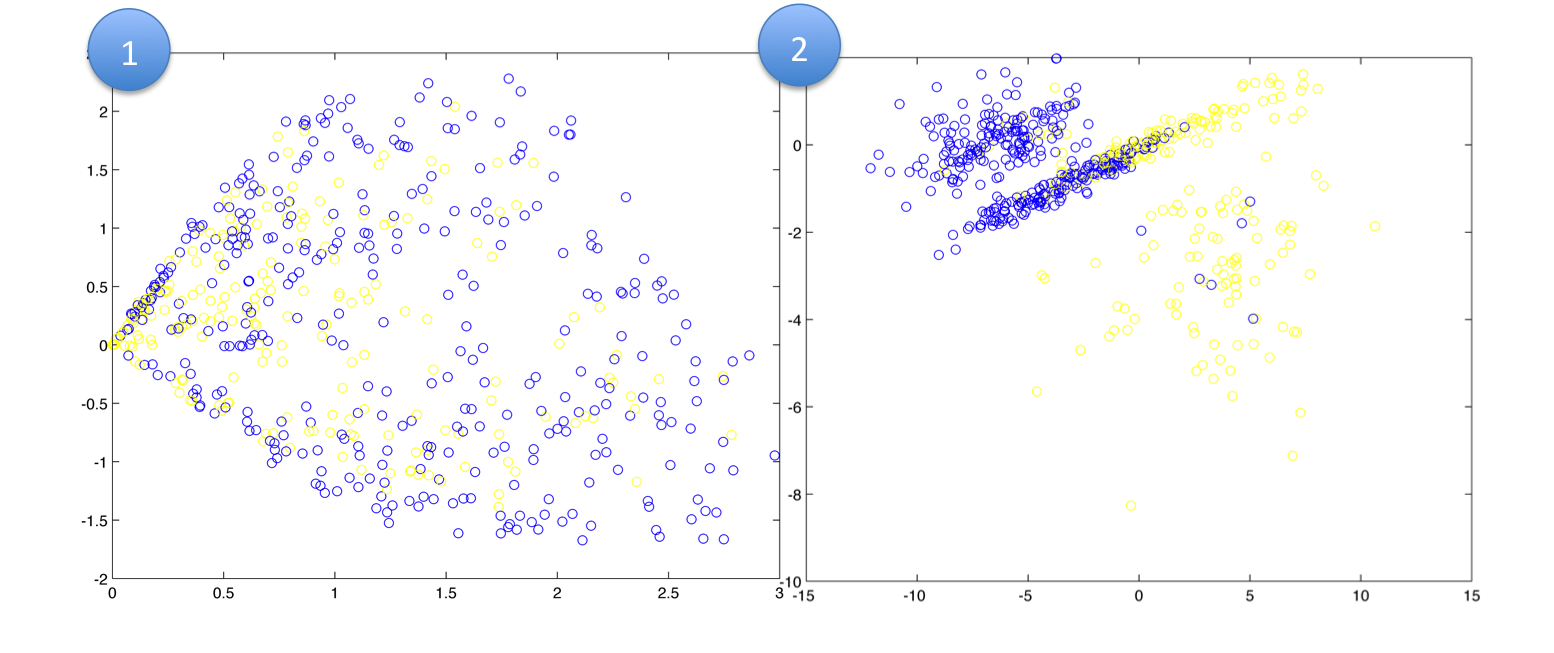
\includegraphics[width=0.7\textwidth]{images/Comparison_PCA_Hidrophila.png}
    \caption{Both images are an made with ML-MS Studio applying PCA analysis with two classes. Figure number one represents PCA technique with only m/z values of selected peaks; figure two represents the PCA analysis made with feature extraction. The blue circles represents A. Hidrophilla samples and the yellow ones are the other samples. (Author 2015).}
\label{fig:pcahidrophilacomparison}
\end{figure}
\subsubsection{A. Trota Results}
On "Trota against all" group we use "Fr. Selected M/Z" feature extraction generating feature with correlation 0.57 and "FR Best Peaks M/Z" with correlation threshold of 0.12, 0.2 and 0.4 generating features with correlation  0.33, 0.11 and 0.68. The PCA comparison with and without feature extraction is represented on figure \ref{fig:pcatrotacomparison}

  \begin{figure}[H]
    \centering
    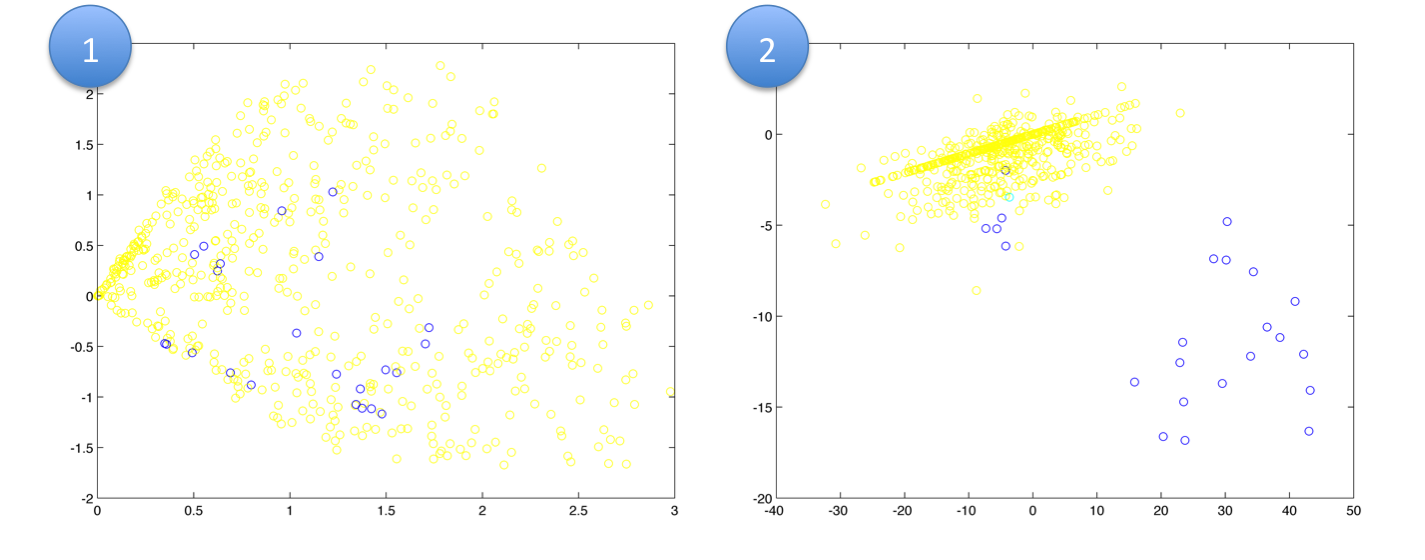
\includegraphics[width=0.7\textwidth]{images/Comparison_Trota_PCA.png}
    \caption{Both images are an made with ML-MS Studio applying PCA analysis with two classes. Figure number one represents PCA technique with only m/z values of selected peaks; figure two represents the PCA analysis made with feature extraction. The blue circles represents A. Trota samples and the yellow ones are the other samples. (Author 2015).}
\label{fig:pcatrotacomparison}
\end{figure}


\section{References}



\bibliographystyle{elsarticle-num} 
\bibliography{mendeley.bib}


%% else use the following coding to input the bibitems directly in the
%% TeX file.

%%\begin{thebibliography}{00}

%% \bibitem{label}
%% Text of bibliographic item

%%\bibitem{}

%\end{thebibliography}
\end{document}
\endinput
%%
%% End of file `elsarticle-template-num.tex'.
